\documentclass[11pt]{article}

\usepackage[margin=1in]{geometry}
\usepackage{amsmath}
\usepackage{amssymb}
\usepackage{amsthm}
\usepackage[ruled,vlined,linesnumbered]{algorithm2e}
\usepackage{tikz}
\usepackage{graphicx}
\usepackage{cite}
\usepackage{float}
\usepackage{hyperref}
\SetArgSty{textnormal}

\input{macros.tex}

\newtheorem{theorem}{Theorem}[section]
\newtheorem{lemma}[theorem]{Lemma}
\newtheorem{corollary}[theorem]{Corollary}
\theoremstyle{definition}
\newtheorem{observation}[theorem]{Observation}
\newtheorem{proposition}[theorem]{Proposition}

\newcommand{\cut}{\delta}
\newcommand{\Etree}{\mathbb{E}_{T\sim\mu}}

\title{Graph Partitioning with Demands: Generalized Graph Conductance With Applications to Hierarchical Clustering}
\author{Micha{\l} Szyfelbein \\ Gda\'nsk University of Technology \and Dariusz Dereniowski \\ Gda\'nsk University of Technology}
\date{\today}

\begin{document}

\maketitle

\begin{abstract}
  In this work, we study various graph partitioning problems under a general demand model. In each such task, we are given a graph $G=(V,E,c,w)$ with a capacity function $c\colon E\to \mathbb{N}$ and a demand function $w\colon V\times V\to \mathbb{N}$. Our main focus is the problem of finding a cut $(S, \bar{S})$ minimizing the quantity
  \[
  \psi_w( S ) = \frac{c( S, \bar{S} )}{w( S, V )\cdot w( \bar{S}, V )}.
  \]
  Here, $c( S, \bar{S} )$ is the cost of edges between $S$ and the complement of $S$, $\bar{S}$, and $w( S, V )=w( S )+w( S, \bar{S} )$ is the sum of the internal demand within $S$, $w( S )$, and the demand between vertices of $S$ and $\bar{S}$, $w( S, \bar{S} )$. We call $\psi_w( S )$ the \emph{generalized conductance} of the cut $(S, \bar{S})$, and the task of minimizing $\psi_w( S )$ the \textsc{Generalized Conductance Problem}. Our main contribution is an algorithm with an $\mathcal{O}(\log n)$-approximation guarantee for this objective. Our result is achieved via a two-way reduction: first to the well-known \textsc{Generalized $k$-Multicut Problem}, and then to a constrained variant of the classic \textsc{Sparsest-Cut Problem}, with an additional upper-bound constraint on the amount of demand that may be cut.
  
  Moreover, we show that the above procedure can be leveraged to obtain an $\mathcal{O}(\log n)$-bicriteria approximation for \textsc{Graph Partitioning with Demands}, where the goal is to find a minimum-cost subset of edges $C$ such that for every component $H$ of $G\setminus C$, $w( H )\leq \rho\cdot w( V )$. This, in turn, yields an $\mathcal{O}(\log n)$-approximation for \textsc{Hierarchical Clustering with Demands}, the problem of finding a hierarchy of cuts that partitions the graph into increasingly refined clusters. For multiplicative demand functions, our framework improves these guarantees to $\mathcal{O}(\sqrt{\log n})$ and for trees we obtain an $\mathcal{O}(1)$-approximation for all of the above objectives.
\end{abstract}

\noindent\textbf{Keywords:} Graph partitioning with demands, Generalized conductance, Sparsest cut, Generalized multicut, Hierarchical clustering, Approximation algorithms.


\section{Introduction}

Sparsest cut is a central problem among various graph partitioning tasks. Given a graph $G=(V,E, c)$, where $c\colon E \to \mathbb{N}$ is a capacity function, the goal is to find a subset of vertices $S\subseteq V$ that minimizes

\[
\phi\br{S} = \frac{c\br{S, \bar{S}}}{\spr{S}\cdot \spr{\bar{S}}}.
\]
where $\bar{S}=V\setminus S$ and $c\br{S,\bar{S}}=\sum_{u\in S}\sum_{v \in \bar{S}}c\br{u, v}$.

This problem has been extensively studied in the literature resulting in remarkable connections to topics including metric spaces and spectral graph theory with the state-of-the-art approximation algorithm due to Arora, Rao, and Vazirani \cite{ExpanderFlowsGeometricEmbeddingsAndGraphPartitioning}, achieving an approximation ratio of $\bigo\br{\sqrt{\log n}}$, where $n=\spr{V}$. Moreover, it also has a number of applications as an essential primitive in other graph algorithms, where it serves as a building block for various divide-and-conquer strategies. This includes graph partitioning where the goal is to find a subset of edges of minimum capacity such that all of the connected components resulting from deleting these edges are of small size. Another example is the problem of hierarchical clustering with similarity measures, where the goal is to hierarchically cluster data points, so that to minimize the Dasgupta's clustering objective. Intuitively, this objective promotes clusters with both children of balanced size as well as a low capacity of edges cut between them. In particular, given an $\alpha$-approximation algorithm for the sparsest cut, one can obtain an $\bigo\br{\alpha}$-approximation algorithm for both of the aforementioned problems \cite{ExpanderFlowsGeometricEmbeddingsAndGraphPartitioning,HierarchicalClusteringObjectiveFunctionsAndAlgorithms,ApproximateHierarchicalClusteringViaSparsestCutAndSpreadingMetrics}.

This usefulness of sparsest cut can be attributed to the following observation, implicitly exploited by many algorithms.
The quantity $\spr{S}\cdot \spr{\bar{S}}$ can be interpreted in two separate ways. First, imagine each pair of vertices to be associated with a unit demand. Then, $\spr{S}\cdot \spr{\bar{S}}$ can be seen as the total demand crossing the cut. This interpretation is useful for the sake of developing approximation algorithms for the sparsest cut itself, since a weak duality between sparsest cut and multicommodity flow type problems has been established \DD{[tutaj by sie przydalo cytowanie, jesli mozliwe]}. Secondly, $\spr{S}\cdot \spr{\bar{S}}$ can be observed to be large when both partitions are of roughly equal size. This comes useful when developing divide and conquer algorithms for other graph problems, since the product in the denominator becomes a measure of the balance of a cut.

However, if one were to generalize the sparsest-cut to general demands setting, these two interpretations are no longer equivalent. Let $w\colon V\times V\to \mathbb{N}$ be a demand function.
The \emph{generalized sparsest cut problem} \DD{usunalem ``with demands'' gdyz dalej tak bylo} is to find a subset of vertices $S\subseteq V$ that minimizes
\[\phi_w\br{S} = \frac{c\br{S, \bar{S}}}{w\br{S, \bar{S}}}.
\]
This problem is also well-understood, and the state-of-the-art approximation algorithm is due to Arora, Lee, and Naor \cite{EuclideanDistortionAndTheSparsestCut}, which achieves the ratio of $\bigo\br{\sqrt{\log n}\cdot \log \log n}$. However, as discussed above, in order to use the some notion related to sparsity in a wider range of applications, it would be desirable to approximate some quantity measuring the balance of a cut. 
To the best of our knowledge, no such results have been obtained in the literature yet.
The graph \emph{conductance} is a well-known measure of the balance of a cut, defined as
\[
\phi\br{S} = \frac{c\br{S, \bar{S}}}{\operatorname{vol}(S)\cdot \operatorname{vol}(\bar{S})}.
\]
where $\operatorname{vol}(S)=\spr{\brc{e\in E\colon e\cap S\neq \emptyset}}$\footnote{Note, that there are several similar definitions of the conductance, however they are all equivalent up to constant factors.}. In fact, for the case of unit demands, the conductance is equivalent to the sparsest cut, up to a constant factor. However, for the general demands this is not a case, and this will come useful in our applications. The \emph{generalized conductance} of a cut $\br{S,\bar{S}}$ will be, defined as
\[
\psi_w\br{S} = \frac{c\br{S, \bar{S}}}{w\br{S, V}\cdot w\br{\bar{S}, V}}.
\]
The problem of $\psi_w$ minimization will be called the \emph{minimum generalized conductance} problem.
\DD{tutaj usunalem powtorzenie, ze to nie bylo studiowane (zwlaszcza, ze piszemy, ``we introduce ...'' powyzej}
%To the best of our knowledge, this objective has not been studied in the literature yet, and it is not known whether it admits an algorithm with a non-trivial approximation ratio.
We initiate the study of this problem by providing an $\bigo\br{\log n}$-approximation algorithm for general graphs.
Interestingely enough, in our algorithm we use a non-trivial reduction to the former generalized sparsest cut with demands, i.e., the minimization of $\phi_w$.
\DD{dalej uproscilem, gdyz bez definicji robi sie to za malo formalne chyba. A za chwile i tak wszystko bedzie w ``our results''.}
%However, in order for the approximation ratio to be preserved, \DD{powyzsze nie wskazuje, ze ``zachowujemy'' app. ratio, a raczej dostajemy nieco gorsze} additional constraint expressing the maximum amount of demand cut is required. We call this problem a constrained sparsest cut problem and show, how to solve it using
At the core of our method are algorithmic reductions to few cut-like problem, including the one just mentioned as an example, and the notion of
cut-sparsifier tree decompositions by R\"{a}cke \cite{OptimalHierarchicalDecompositionsForCongestionMinimizationInNetworks}.
%Since the embedding \DD{piszac ``the'' embedding odnosimy sie do kontekstu, ale nie jest jasne jaki embedding mamy na mysli.} step incurses an $\bigo\br{\log n}$ distortion and one can the constrained sparsest cut on trees in polynomial time, we get the desired approximation ratio.

%It should be noted, that this is not the only possible balance-oriented generalization of the sparsest cut. For instance, one could also consider the following ratio:
% \[
% \psi'_w\br{S} = \frac{c\br{S, \bar{S}}}{w\br{S}\cdot w\br{\bar{S}}}.
% \]
%However, the first objective $\psi_w\br{S}$ is more natural due to the fact that it also takes into account the demands crossing the cut, since $w\br{S, V}= w\br{S}+w\br{S, \bar{S}}$. As it turns out, this becomes crucial for the applications we have in mind, and thus we focus on $\psi_w\br{S}$.
\DD{mam mieszane odczucia, czy ta koncowka wiecej nie namiesza niz pomoze. Otwiera bowiem watpliwosc czy nie jest sytuacja taka, ze studiuje sie wybrany sobie jeden wariant z wielu i recenzent sie zacznie zastanawiac dlaczego ten jest lepszy niz inny. Trzymalbym sie zatem narracji: po pierwsze uogolnienie, wiec dobrze, po drugie problem nietrywialny, wiec dobrze; po trzecie jest naturalna interpretacja; po czwarte uzyteczny. Tu by byla kropka. Chodzi o to, ze ludzie czesto sa oporni do prac wprowadzajacych nowy problem, gdyz sa cale morza prac, ktore to czynia i wiekszosc tych podproblemow i wariantow zwyczajnie nie jest zbyt ciekawa (lub interasujaca dla waskiego grona). Na razie zakomentowalem.
Moze do podsumowania taka dyskusja?}

\subsection{Our results and techniques}

\DD{todo: na razie zosstawilem;}
In this work, we show a series of algorithmic reductions between a large number of problems. The generalized conductances turns out to be the central one of them. Due to this we structure our work into two main parts.

Firstly, we concern ourselves with approximating the latter problem. To do so, we combine a variety of techniques in order to simplify the problem. Intuitively, our algorithm is sensitive to two types of instances which are tackled differentily. Although our algorithm never distinguishes between them explicitly, by choosing the best among two obtained solutions we get a non-trivial approximation ratio of $\bigo\br{\log n}$. The two cases are dictated by the size of $w\br{S, \bar{S}}$. If this quantity is large enough, then the problem (up to a constant factor approximation loss) essentially becomes the well known $k$-multicut problem, where the task is to minimize the cost of cut edges while ensuring that at least $k$ unit of demands are partitioned. The only difference is that here the number of connected components outputed by the algorithm might be arbitrarily large. To remedy this we employ a max-cut algorithm which ensures that a significant portion of the demand is still cut while partitioning the components into two groups as required.

If the aforementioned quantity is small, then we show that we can reduce the problem to the classic sparsest-cut with additional constraint that the demand cut cannot be too large. This is done by constructing an auxiliary graph with new demand function such that cutting demand in this new instance roughly corresponds to minimizing the conductance in the original instance. This reduction preserves the approximation ratio, however its analysis is sensitive and crucially relies on the fact that $w\br{S, \bar{S}}$ is assumed to be of small value. 

In order to tackle this constrained version of the sparsest cut we use a general technique by \cite{OptimalHierarchicalDecompositionsForCongestionMinimizationInNetworks}. The idea is to embed a graph into a polynomial-sized convex combination of trees, which in expectance preserves the value of any cut up to $\bigo\br{\log n}$ distortion. This allows us to obtain the $\bigo\br{\log n}$-approximation by solving the problem to optimality on all trees and outputting the best of the solutions. This indeed becomes an easy task, since the (unconstrained) sparsest cut can be found in a tree by only considering cuts with singular edge cut. As it turns out, the same is true for the constrained version of the problem.

\DD{todo: tutaj skleic...} This problem admits an $\beta=\bigo\br{\log n}$-approximation algorithm by combining \cite{AUnifiedApproachToApproximatingPartialCoveringProblems} with \cite{OptimalHierarchicalDecompositionsForCongestionMinimizationInNetworks}.
\DD{to by moze poszlo do frontu do our results:}
\begin{corollary}
  There is a polynomial-time $O(\log n)$-approximation algorithm for the problem of minimizing $\psi_w\br{G}$ on general graphs as well as an $O(1)$-approximation algorithm for the problem of minimizing $\psi_w\br{G}$ on trees.
\end{corollary}

In the second part of the paper we move ourselves towards applications of the generalized conductance. We show that by iterative application of the above algorithm we can partition the graph into components with demand at most $\frac{4}{5}\cdot w\br{V}$ while paying only $\bigo\br{\log n}$ times more than it is required to partition the graph into components with demand at most $w\br{V}/2$. Therefore, the algorithm is a bicriteria approximation.
% It should be noted, that there is an evidence that no true polylogarithmic approximation for this task exists [cite here].

Then, we show that the above bicriteria approximation algorithm can be used to obtain an $\bigo\br{\log n}$-approximation for hierarchical clustering with demands. This is done in a recursive top-down manner. The algorithm starts by finding a graph partition consisting of components with demand at most $\frac{4}{5}\cdot w\br{V}$. Then, the rest of hierarchy is build by applying the algorithm recursively in all of the resulting clusters. Using a tight analysis generalizing the framework of \cite{ApproximateHierarchicalClusteringViaSparsestCutAndSpreadingMetrics} we show that the approximation ratio is indeed preserved.

Figure \ref{fig:reductions} shows the algorithmic reductions that appear in this work.

\begin{figure}[H]
  \centering
  \resizebox{\textwidth}{!}{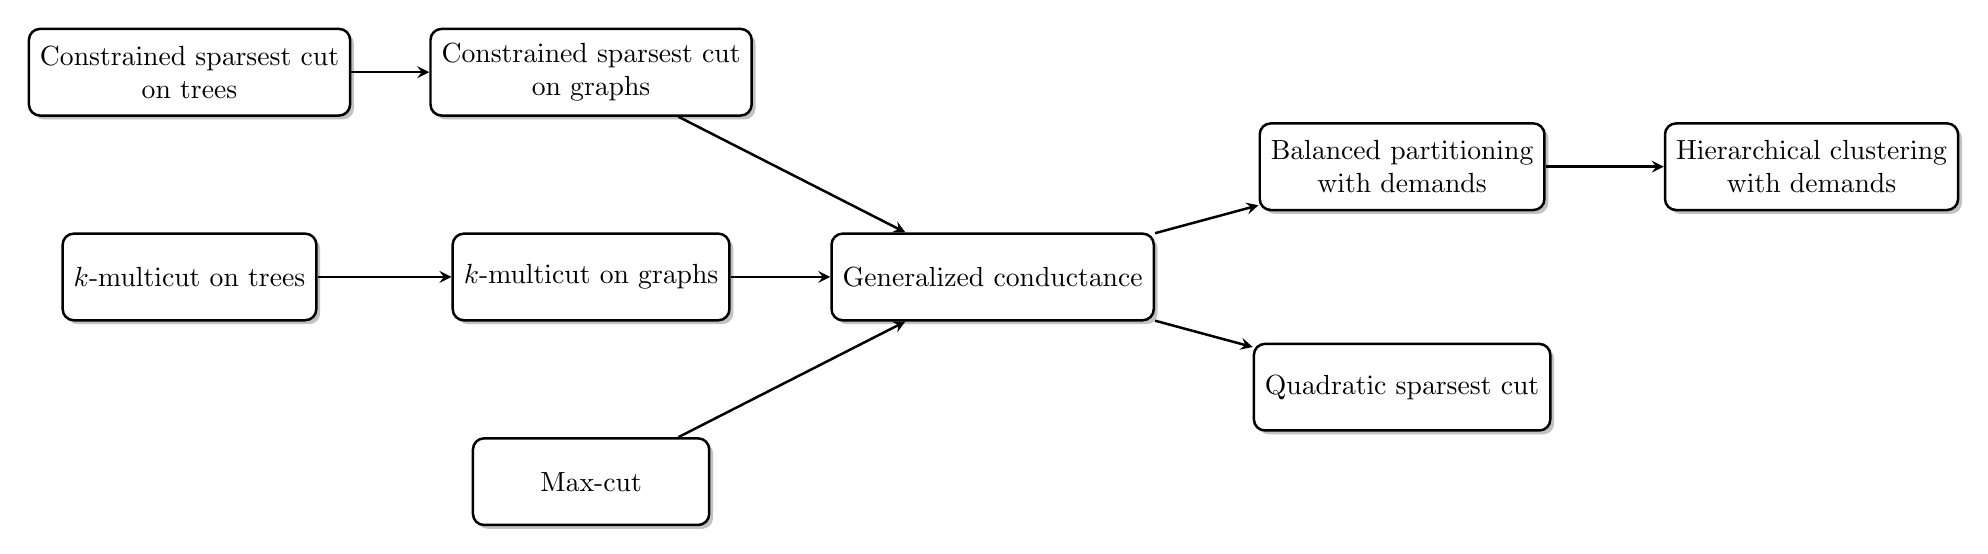
\begin{tikzpicture}[>=stealth, line width=0.9pt]
  \tikzstyle{box}=[draw, rounded corners, align=center, inner sep=4pt,
    minimum width=3cm, minimum height=1.10cm,
    fill=white,
    preaction={fill=black,opacity=0.24,transform canvas={xshift=1.4pt,yshift=-1.4pt}}]

  % Left: tree problems
  \node[box] (cst) at (0, 2.6) {Constrained sparsest cut\\on trees};
  \node[box] (kmt) at (0, 0.0) {$k$-multicut on trees};

  % Middle-left: graph problems + max-cut
  \node[box] (csg) at (5.1, 2.6) {Constrained sparsest cut\\on graphs};
  \node[box] (kmg) at (5.1, 0.0) {$k$-multicut on graphs};
  \node[box] (mc)  at (5.1, -2.6) {Max-cut};

  % Center: target problem
  \node[box, minimum width=3cm] (gc) at (10.2, 0.0) {Generalized conductance};

  % Right: applications
  \node[box] (bpd) at (15.4, 1.4) {Balanced partitioning\\with demands};
  \node[box] (qsc) at (15.4, -1.4) {Quadratic sparsest cut};
  \node[box] (hcd) at (20.6, 1.4) {Hierarchical clustering\\with demands};

  \draw[->] (cst) -- (csg);
  \draw[->] (kmt) -- (kmg);

  \draw[->] (csg) -- (gc);
  \draw[->] (kmg) -- (gc);
  \draw[->] (mc)  -- (gc);

  \draw[->] (gc) -- (bpd);
  \draw[->] (gc) -- (qsc);
  \draw[->] (bpd) -- (hcd);
\end{tikzpicture}
}
  \caption{Reduction map of problems and applications considered in this paper.}
  \label{fig:reductions}
\end{figure}
\subsection{Related work}


\section{Preliminaries}

\DD{uklad preliminaries: pierwszy paragraf to definicje ogolno-grafowe, a drugi to cuty, demandy i ich notacja.}

Most of the instances of the problem considered in this work consist of a graph $G=\br{V,E,c,w}$, where $V$ is the vertex set, $E$ is the edge set, $c\colon E \to \mathbb{N}$ is the \emph{capacity} function which encodes the cost of cutting an edge, and $w\colon V\times V\to \mathbb{N}$ is the \emph{demand} function which, informally speaking, tells how important separating a given vertex pair is.
For adjacent vertices $u,v\in V$, we denote by $uv$ the edge between $u$ and $v$.
For any $C\subseteq E$, $G-C$ is the graph obtained by removing the edges in $C$ from $G$.
We write $\br{V_H,E_H,c_H,w_H}$ to point out that given parameters represent a particular graph or subgraph $H$, different than $G$.

For any function $f\colon V\times V\to \mathbb{N}$ and \DD{usunalem ``disjoint'' ...} subsets $A, B\subseteq V$, we define:
\[
f\br{A}=\sum_{u,v\in A}f\br{u, v}, \quad f\br{A, B}=\sum_{u\in A}\sum_{v\in B}f\br{u, v}
\]
with a convention that if the domain of $f$ is the edge set and $uv\notin E$, then $f\br{u,v}=0$.
Note that whenever $A, B\subseteq V$ are not disjoint, \DD{... i wtedy to jest konsekwencja tej definicji powyzej.} we have $f\br{A, B}=f\br{A}+f\br{A, B\setminus A}$.
For a subset $C\subseteq E$ and a function $f$ on the edge set, $f\br{C}=\sum_{uv\in C}f\br{u,v}$.
\DD{todo: czy zdarza sie, ze mamy funkcje zdefiniowana na $V\times V$, ale argumentem jest zbior krawedzi?}
For a subset $S\subseteq V$, we denote by $\bar{S}$ the complement of $S$ in $V$, i.~e. $\bar{S}=V\setminus S$.
A \emph{cut} is any subset $S\subseteq V$, such that $S\neq \emptyset$, $S\neq V$ and we denote it either by just $S$ or we write $\br{S, \bar{S}}$ to explicitly indicate the two sides of the cut.
It will be sometimes more convienient to call a cut the set of edges having one endpoint in $S$ and the other in $\bar{S}$.
Which definition is used will be clear from the context.
We define the demand \emph{cut} by a subset of edges $C\subseteq E$ to be the sum of all $w(u,v)$ such that $u$ and $v$ belong to different connected components of $G-C$.

\section{The main algorithm}

In order to tackle the minimum generalized conductance problem, our first objective is to further simplify the denominator $w\br{S, V}\cdot w\br{\bar{S}, V}$ into a linear function. We may without loss of generality assume that $w\br{S, V}\le w\br{\bar{S}, V}$.
Consequently, $w\br{V}/2\leq w\br{\bar{S}, V} \leq w\br{V}$ and thus, minimizing $\psi_w\br{S}$ is equivalent to minimization of
\[h_w\br{S}=\frac{c\br{S, \bar{S}}}{w\br{S, V}}, \quad \text{subject to} \quad w\br{S, V}\le w\br{\bar{S}, V}\] up to a constant factor loss. 
\DD{TODO: jeszcze moze dodac intuicje o tej stalej.}

However, for our purposes we will slightly relax the assumption that $w\br{S, V}\le w\br{\bar{S}, V}$ and in turn we will only require that $w\br{S, V}\le \C\cdot w\br{\bar{S}, V}$ for some appropriate constant $\C>1$.
\DD{$c$ juz jest zajeta na capacity, wiec zmienilem stala na $\C$ (uwaga: jest to makro, wiec mozna przedefiniowac).}
This still preserves the approximation ratio up to a factor dependent on $\C$ by a similar discussion.

As an internal tool used in this section we will utilize the generalized $k$-multicut problem, which is as follows.
Given a graph $G=(V,E,c,w)$ with capacities and demands, the \emph{generalized $k$-multicut problem} is to find a minimal-cost set of edges $C\subseteq E$, such that the demand cut by $C$ is at least $k$.

We now introduce a reduction\footnote{We use the word `reduction' since both $S_1$ and $S_2$ are obtained via an algorithmic reduction to another combinatorial problem, either generalized sparsest cut (with restrictions) or the generalized $k$-multicut.} scheme used in this section.
The scheme is applied to an input graph $G=(V,E,c_G,w_G)$ and it computes independently two candidate sets $S_1$ and $S_2$ via two different methos.
The returned solution is $S_i$ that minimizes $\psi_w$.
Formally, the scheme is the following:
\begin{enumerate}
  \item \label{it:S1} Compute a candidate set $S_1$:
  \begin{enumerate}[label=(\theenumi\alph*)]
    \item\label{it:S1:Gprime} Build an auxiliary graph $G'=(V',E',w_{G'},c_{G'})$ by adding a universal vertex $r$, i.e. $V'=V\cup\brc{r}$ and $E'=E\cup\brc{ru\colon u\in V}$, setting the capacities to $c_{G'}\br{r,u}=0$ for each $u\in V$ and $c_{G'}\brc{u,v}=c_G\brc{u,v}$ for each $u,v\in V$, and the demands to $w_{G'}\br{r,u}=\sum_{v\in V}w_G\br{u,v}$ for each $u\in V$ and $w_{G'}\br{u,v}=0$ for each pair $u,v\in V$.
    \item\label{it:S1:K} Set $K\gets \frac{4}{3}\cdot w_G\br{V}$.
    \item\label{it:S1:alpha} Run an $\alpha$-approximation algorithm for
    \[
      \min_{S\subseteq V'} \phi_w\br{S}=\frac{c_{G'}\br{S,\bar S}}{w_{G'}\br{S,\bar S}}
      \quad\text{subject to}\quad 0<w_{G'}\br{S,\bar S}\le K.
    \]
    and denote the returned cut by $S_1$. \DD{tutaj zamiast opisywac slownie problem odniosl bym sie, to frazy, ze rozwiazujemy generalized sparsest cut i podac dla jakiej instancji (tak, widze, ze bedzie extra ``subject to''. Jesli to ``subject to'' (nie wiem gdyż czytam liniowo) pojawialoby sie wiecej razy, to pewnie warto nazwac, a jak nie to niech zostanie tak, gdyz jest czytelnie; na razie zostawiam taki marker do oceny pozniej.}
  \end{enumerate}
  \item \label{it:S2} Compute a candidate set $S_2$:
  \begin{enumerate}[label=(\theenumi\alph*)]
    \item Run a $\beta$-approximation algorithm for the generalized $k$-multicut with $k=w_G\br{V}/3$ to obtain a multicut $C$.
    \item Build a complete graph $R$ on components of $G\setminus C$, with edge weights $w_R\br{H_1,H_2}=w_G\br{H_1,H_2}$ for any pair $H_1$ and $H_2$, where $H_1$ and $H_2$ are the vertex set of the components.
    \item Apply rounding: set $W=\frac{w\br{V\br{R}}}{4\cdot \spr{E\br{R}}}$ and replace the weight of each edge \DDfix{$e\in E\br{R}$} by $w'\br{e}=\fl{w\br{e}/W}$.
    \item Run a local search for max-cut on $(R,w')$: start with $(A,B)=(\emptyset,V\br{R})$, repeatedly move a single vertex from $B$ to $A$ if it improves the cut, and stop at a local optimum, i.e., when a single vertex transfer from $B$ to $A$ does not improve the cut.
    \item Map the resulting cut of $R$ back to a cut $S_2$ of $G$.
  \end{enumerate}
  \item Return the better of $S_1,S_2$, i.e., $\argmin_{X\in\brc{S_1,S_2}}\psi_w\br{X}$.
\end{enumerate}

\begin{theorem}
  The above algorithm is an $O\br{\alpha+\beta}$-approximation algorithm for the minimum generalized conductance problem.
\end{theorem}
\begin{proof}

Let $S^*$ be an optimal solution with $w\br{S^*, V}\le w\br{\bar{S}^*, V}$. Our analysis consists of two separate cases depending on the size of $w\br{S^*, \bar{S}^*}$.
We show that no matter what the actual optimal value is, at least one of the $S_i$ gives a good approximation ratio.
Note that the exact choice of constants in our construction is somewhat arbitrary and we do not attempt to optimize them.
\begin{lemma}
  Assume that $w\br{S^*, \bar{S}^*}\leq w\br{V}/3$. %Moreover, let $\alpha$ be an approximation ratio of some approximation algorithm for the problem of minimizing $\phi_w\br{S}$ in $G$ subject to $w_{G}\br{S, \bar{S}}\leq K$.
  Then, $S_1$ is an $O\br{\alpha}$-approximate solution to the minimum generalized conductance problem.
\end{lemma}
\begin{proof}
%To obtain a good approximation for $h\br{S}$, we proceed as follows. Firstly, we create an auxiliary graph $G'$, such that $V'=V\cup \brc{r}$. We set $c\br{r, u}=0$ for every $u\in V$ and we set $w\br{r, u}=\sum_{v\in V} w\br{u, v}$ for every $u\in V$.
Recall the auxiliary graph $G'$ defined in \ref{it:S1:Gprime}.
Take a cut $S\subseteq V$, assuming without loss of generality that $r\in \bar{S}$. We have that:
\[
w_{G}\br{S, V}\leq w_{G}\br{S, V}+w_G\br{S}= w_{G'}\br{S, \bar{S}}\leq 2\cdot w_{G}\br{S, V}
\]
\DD{
czy tu nie powinno byc?:
\[
w_{G}\br{S, V} = w_{G}\br{S, \bar{S}}+w_G\br{S}= w_{G'}\br{S, \bar{S}}\leq 2\cdot w_{G}\br{S, V}
\]
a jesli tak, to da nierownosc zachodzi trywialnie?
}
where the equality is due to the fact that for any $S\subseteq V\br{G'}$, the quanitity $w\br{S, \bar{S}}$ double counts the contribution of edges between the vertices of $S$ in $w_{G}\br{S, V}$.

\DD{tutaj na razie przerywam ten lemat, gdyz mam klopot z czytaniem: ten opis opiera sie sporo na intuicjach stojacych za budowa algorytmu zamiast po prostu policzyc to co jest. Na przyklad pierwszy paragraf budowal graph $G'$ --- dodalem jedno zdanie, zeby czytelnik sobie przypomnial punkt \ref{it:S1:Gprime}. Nastepny paragraf buduje intuicje, ale wydaje sie, ze mowi tylko cos w rodzaju ``Recall the definition of $K$ in \ref{it:S1:K}.''.}
It would be desireable to minimize the value of $\phi_w\br{S} = \frac{c\br{S, \bar{S}}}{w\br{S, \bar{S}}}
$ in this new graph. However, it is also easy to see, that in this new instance a trivial cut $S=V$ has cost $0$. Moreover, we demand $w_G\br{S, V}$ to be roughly smaller then $w_G\br{\bar{S}, V}$. To achieve both ends we thus add the constraint that $w_{G'}\br{S, \bar{S}}\leq K$ for $K=\frac{4}{3}\cdot w_G\br{V}$.

\DD{czemu odwolujemy sie do niezdefiniowanego $h(S)$ w dowodzie?}
We now want to argue that any $\alpha$-approximation of $\phi_w\br{S} $ subject to $w_{G'}\br{S, \bar{S}}\leq K$ in $G'$ is also a good approximation of $h\br{S}$ in $G$. Firstly, observe that for any optimal solution $S^*$ for $h\br{S}$, where $w\br{S^*, V}\leq w\br{\bar{S}^*, V}$ we have that
\[
w_G\br{S^*, V}+w_G\br{\bar{S}^*, V}=w_G\br{V}+w_G\br{S^*, \bar{S}^*}\leq \frac{4}{3}\cdot w_G\br{V}
\]
by our assumption that $w\br{S^*, \bar{S}^*}\leq w\br{V}/3$. As a consequence we get that $w_G\br{S^*, V}\leq \frac{2}{3}w\br{V}.$ In order to move this cut to $G'$ we append $r$ to $\bar{S}^*$.
This gives 
\[w_{G'}\br{S^*, \bar{S}^*}\leq 2\cdot w_G\br{S^*, V}\leq \frac{4}{3}\cdot w_G\br{V}=K.
\]
Therefore, we get that $\br{S^*, \bar{S}^*}$ is a valid solution for $\phi_{G'}\br{S}$ and as a consequence $\phi_{G'}\br{S}\leq h_{G}\br{S}$. Now we want to show an opposite direction, namely, that any solution to the problem of minimizing $\phi_w\br{S}$ in $G'$ subject to $w_{G'}\br{S, \bar{S}}\leq K$ gives a solution for $G$, such that $w_G\br{\bar{S}^*}\geq w\br{V}/6$. By the previous discussion, this yields an $O\br{\alpha}$-approximation for $h\br{S}$ and thus also for $\psi\br{S}$. Let $\br{S_1, \bar{S}_1}$ be the returned partition. 
There are 3 cases:
\begin{enumerate}
  \item $w_{G}\br{S_1, V}\leq \frac{5}{6}\cdot w_G\br{V}$. This means that  \[w_G\br{\bar{S}_1, V}\geq w_G\br{V}-w_{G}\br{S_1, V}\geq w_G\br{V}/6.
  \]
  \item $w_{G}\br{S_1, V}\geq \frac{5}{6}\cdot w_G\br{V}$. There are two subcases:
  \begin{itemize}
    \item $w_G\br{S_1}\geq w_G\br{V}/2$. We get that 
    \[w_G\br{S_1, V}=w_{G'}\br{S_1, \bar{S}_1}-w_G\br{S_1}\leq K-w_G\br{S_1} \leq \frac{4}{3}\cdot w_G\br{V}-w_G\br{V}/2 = \frac{5}{6}\cdot w_G\br{V}.
    \]
    This further means that 
    \[w_G\br{\bar{S}_1, V}\geq w_G\br{V}-w_G\br{S_1, V}\geq w_G\br{V}/6.
    \]
  \item $w_G\br{S_1, \bar{S}_1}\geq w_G\br{V}/3$. Here, we trivially get that $w_G\br{\bar{S}_1, V}\geq w_G\br{S_1, \bar{S}_1}\geq w_G\br{V}/3$.
  \end{itemize}
  It should be noted that at least one of the two above conditions must hold since $w_G\br{S_1}+w_G\br{S, \bar{S}_1}=w_{G}\br{S_1, V}$
\end{enumerate}
The lemma follows.
\end{proof}

Now we analyze, the second case. Here, we use an approximation ratio for  which is as follows: \DD{tutaj skleic...} This problem admits an $\beta=O\br{\log n}$-approximation algorithm by combining \cite{AUnifiedApproachToApproximatingPartialCoveringProblems} with \cite{OptimalHierarchicalDecompositionsForCongestionMinimizationInNetworks}.
\DD{Tw. mowi o tym, ze dostajemy $O(\alpha+\beta)$-approx i nie ma znaczenia ile one wynosza. Jesli chcemy tutaj rozkniniac, ze sa $\log n$-app. to by bylo zasadne, gdyby tw. to mowilo w tresci. Nie sugeruje tego, gdyz konstrukcja black-boxowa jest dobra: tw mowi o arbitralnym $\alpha+\beta$ i dopiero gdzies pozniej dywagacje jakie $\alpha$ i $\beta$ sa osiagalne i nastepnie finalny wspolczynnik. Natomiast poprzednie zdanie jest zbedne dla tego dowodu (moze to umnkelo, ale jestesmy w srodku dowodu twierdzenia).}
\begin{lemma}
  Assume that $w\br{S^*, \bar{S}^*}\geq w\br{V}/3$.
  %Moreover, let $\beta$ be an approximation ratio of some approximation algorithm for the (generalized) $k$-multicut problem.
  \DD{usunalem zalozenie o $\beta$, gdy to juz jest zdefiniowane w algo, a jesli chcemy w claimach przywolac, to jesli lematy sa zagniezdzone, to raczej w twierdzeniu.}
  Then, $S_2$ is an $O\br{\beta}$-approximate solution to the minimum generalized conductance problem.
\end{lemma}
\begin{proof}
  In this case, we have that $w\br{S^*, V}, w\br{\bar{S}^*, V}=\Theta\br{w\br{V}}$ \DD{w sumie tego nie widac, wiec dobrze byloby rozpisac/uzasadnic chocby jednym zdaniem} and therefore with a constant factor loss, it suffices to minimize $c\br{S, \bar{S}}$ subject to $w\br{S, \bar{S}}\geq w\br{V}/3$. \DD{tutaj dobrze byloby byc dokladniejszym co mamy na mysli: czy mamy const-factor loss wzgledem najlepszego rozwiazania, ktore spelnia $w\br{S, \bar{S}}\geq w\br{V}/3$ (i moze takie rozwiazanie jest gorsze od optimum bez tego ograniczenia), czy moze chodzi o to, ze zakladamy, ze input instance jest szczegolna i spelnia $w\br{S, \bar{S}}\geq w\br{V}/3$ i wtedy mamy const-factor loss wzgldem prawdziwego optimum dla takiej instancji?}
  Notably, this task is not equivalent to the $k$-multicut problem since $G\setminus C$ might consist of more then two components. To remedy this issue we proceeed as follows:
  \DD{mysle, ze raczej nalezaloby przerobic ten dowod, gdyz jest bardziej opisem algorytmu, natomiast klarowniej byloby tylko zrobic rachunki dajac ref-y do punktow algorytmu (zaproponowalem tam labele), aby czytelnik mogl spojrzec na algorytm i widziec ktory jego krok jest w danym momencie przeliczany.}
  We find an $\beta$-approximate multicut $C$. Then, we build a complete graph $R$, on vertex set consisting of components of $G\setminus C$. For any $H_1, H_2\in G\setminus C$, we set a weight $w_R\br{H_1, H_2}=w_G\br{H_1, H_2}$ (be weary of the fact that $H_1, H_2$ are vertices of $R$, but subsets of vertices of $G$). We now wish to solve a max-cut problem on $R$ in order to partition components of $G\setminus C$ in such a way to preserve a significant amount of demand being cut. Given a graph $R$, with weights $w$, the max-cut is to find a partition $\br{S_R, \bar{S_R}}$ of $V\br{R}$, such that $w\br{S_R, \bar{S_R}}$ is maximized. Although max-cut is NP-hard, it is well known that for any graph, there exists a cut $\br{A, B}$, such that $w\br{A, B}\geq w\br{V\br{R}}/2$. It is easy to see, that such a solution is $2$-approximation for max-cut, however for our purposes the crucial property is that since the demand cut by $C^*$ is at least $w_R\br{V\br{R}}=w_G\br{V}/3$, finding $(A, B)$ produces a cut of $G$ cutting at least $w\br{V}/6$ amount of demand which is sufficient for our purposes.
  
  To find an appropriate cut, we need an additional detail regarding the runtime of the our algorithm. There exists a local search policy which finds $\br{A, B}$ however its running time is pseudopolynomial in the weights.
  \DD{tutaj widac o co mi chodzilo: dowod musi uzupelniac algorytm. Parafrazujac o co mi chodzi: albo w typowym schemacie opis algorytmu i w dowodzie tylko analiza, albo zwyczajowo lemma mowi, ze cos da sie obliczyc i w dowodzie jest zaszyty algorytm. Tutaj mamy troche mix, oraz powtorzenia. Powtorzenia, gdyz sa zdania, ktore mowia co algorytm robi po kolei. Z drugiej strony sa uzupelnienia algorytmu. To drugie chyba jeszcze mogloby byc, choc pwnie lepiej byloby wyekstrachowac jakis lemat o local search mowiacy jak to zrobic i w jakim czasie i dac to jako cos niezaleznego poza tymi lematami i tym twierdzeniem (globalny lemat). Dodatkowe zamieszanie jest takie, ze analizujemy czas dzialania, wiec w tresci tw. trzebaby dodac, ze algorytm jest wielomianowy. Albo: ten globalny lemat powyzej moze moglby mowic, ze powyzszy schemat algorytmiczny dziala w wielomianoym czasie i tam przerzucic te kwestie zlozonosciowe.}
  To mitigate this inconvenience we perform a knapsack-like rounding step first. Let $W=\frac{w\br{V\br{R}}}{4\cdot \spr{E\br{R}}}$. For any $e\in E\br{R}$ we set $w'\br{e}=\fl{\frac{w\br{e}}{P}}$. Let $\br{A', B'}$ be the cut in this new instance for which $w'\br{A', B'}\geq w'\br{V\br{R}}/2$. For any edge $e$, $W\cdot w'\br{e}$ might be smaller then $w\br{e}$, but by no more then by $W$ (additively). Thus, by summing up over all edges cut by $\br{A, B}$ we get that:
\[
w\br{A, B}-W\cdot w'\br{e}\leq \spr{E\br{A, B}}\cdot W\leq \spr{E\br{R}}\cdot W.
\]
We have:
\[
w\br{A', B'}\geq W\cdot w'\br{A, B}\geq w\br{A, B} - \spr{E\br{R}}\cdot W = w\br{A, B}-w\br{V\br{R}}/4\geq w\br{V\br{R}}/4
\] 
We conclude that finding $\br{A', B'}$ gives us a cut of $R$ cutting at least $w\br{V\br{R}}/4$ amount of demand, which is still sufficient for out purposes.
Moreover, we have that 
\[
w'\br{V\br{R}}=\sum_{e\in E\br{R}}w'\br{e}\leq \frac{1}{W}\cdot \sum_{e\in E\br{R}}w\br{e}=4\spr{E\br{R}}^2
.\]
Hence, there are polynomially many values, that any cut of $\br{R, w'}$ can take, which will certify the polynomial runtime of our procedure.

In order to find $(A',B')$, we use the aforementioned local-search heurstic which is as follows: Start with $A=\emptyset, B=V\br{R}$. At any iteration, consider each vertex $v\in V\br{R}$, and if swapping the assignment of $v$ between $A$ and $B$ results in a better cut, perform the swap. Proceed until no such improvement is possible. For any vertex $v\in V\br{R}$, denote by $w'\br{v}$ its contribution to $w'\br{A', B'}$. We have the following:
\begin{align*}
2w'\br{A', B'}&=\sum_{v\in A'}w'\br{v}+\sum_{v\in B'}w'\br{v}
\\&\geq 
\sum_{v\in A'}\frac{w'\br{v, V\br{R}}}{2}+\sum_{v\in B'}\frac{w'\br{v, V\br{R}}}{2}
\\&=
\frac{1}{2}\sum_{v\in V\br{R}}w'\br{v, V\br{R}}=w'\br{V\br{R}}
\end{align*}
where the inequality is by the halting condition of our procedure.

The running time is polynomial, since every swap increases the weight of the cut, which as argued above can only take polynomially many different values.

Upon finding $\br{A', B'}$ we output the partition $\br{S_2, \bar{S}_2}$ of $V\br{G}$, such that vertices of members of $A'$ belong to $S_2$ and vertices of members of $B'$ belong to $\bar{S}_2$. We have that we cut at least $w\br{V}/12$ amount of demand, and the cost of the edges cut is $c\br{S_2, \bar{S}_2}\leq c\br{C}$, since $E\br{S_2, \bar{S}_2}\subseteq C$.
\end{proof}

By picking the best among the two created solution we ensure that the approximation ratio of the above procedure is upper bounded by $O\br{\alpha+\beta}$.
\end{proof}

Therefore it remains to obtain an approximation algorithm for the problem of minimizing $\phi_w\br{S}$ subject to $w\br{S, V}\leq K$, i.e., the algorithm used in step~\ref{it:S1:alpha}.
In what follows, we show how to do this using cut-sparsifier tree decompositions. We have the following proposition: \DD{czy to z literatury czy tuta? Jesli z lit. to trzebaby [??] dodać. Ogólnie dwuznaczna fraza jest ``subject to exact ...'': po pierwsze te claimy powinny mowic ``polynomial-time''; po drugie ten exact alg. for trees to trzebay napisac dla jakiego problemu, gdyz zaglujemy tutaj szeregiem problemow.}
\begin{proposition}
  There exists an $\alpha=O\br{\log n}$-approximation algorithm for the $\phi_w\br{S}$ subject to $w\br{S, V}\leq K$ problem
   for general graphs and an exact algorithm for trees.
\end{proposition}

It should be noted that the $O\br{\log n}$-approximation algorithm for the generalized $k$-multicut is also obtained using cut-sparsifiers \DD{domyslam sie, ze moze tutaj miec miejsce forward-referencja do innych miejsc. Trzeba dopilnowac, ze jesli uzywamy cos czego zrobimy to ze dla czytelnika to jest jasne i ze jasne jest to jakie brzmienie ma fakt, ktory uzywamy} in conjunction with an $O\br{1}$-approximation algorithm for trees. By combining all of the above discussions, we get the following corollary:
\begin{corollary}
  There is a polynomial-time $O(\log n)$-approximation algorithm for the problem of minimizing $\psi_w\br{G}$ on general graphs as well as an $O(1)$-approximation algorithm for the problem of minimizing $\psi_w\br{G}$ on trees.
\end{corollary}

A special kind of demand function is one, where for each vertex there exists a potential function $\pi\colon V\to \mathbb{N}$, such that for every $u,v\in V$, $w\br{u,v}=\pi\br{u}\cdot \pi\br{v}$. We call such a function a \emph{multiplicative function}. Notably, unit demand is multiplicative with $\pi\br{u}=1$ for every $u\in V$. For such demand functions, we have the following strengthening of approximation guarantees:
\begin{theorem}
  If the demand function $w$ is multiplicative, then there is a polynomial-time $O\br{\sqrt{\log n}}$-approximation algorithm for the problem of minimizing $\psi_w\br{S}$.
\end{theorem}
\begin{proof}
  Firstly, assume that $\pi\br{S}\leq \pi\br{\bar{S}}$. Since for multiplicative demands we have 
  \[
  w\br{A, B}=\sum_{u\in A}w\br{u}\cdot \sum_{v\in B}w\br{v}= \pi\br{A}\cdot \pi\br{B}
  \] 
  we get that $w\br{S, V}\leq w\br{\bar{S}, V}$ and moreover $w\br{S}\leq w\br{S, \bar{S}}$. Thus, minimizing $\psi_w\br{G}$ is up to a constant factor equivalent to minimizing 
  \[\frac{c\br{S, \bar{S}}}{w\br{S, \bar{S}}}=\frac{c\br{S, \bar{S}}}{\pi\br{S}\cdot \pi\br{\bar{S}}}.
  \]
  This can be then reduced to the min-ratio vertex cut problem which is as follows: Given a graph $G=\br{V,E,c,\omega}$, with a capacity vertex function $c\colon V\to \mathbb{N}$ and weight function $\omega\colon V\to \mathbb{N}$ find a partition $A, S, B$ of $V$ that minimizes 
  \[\frac{c\br{S}}{\omega\br{A\cup S}\cdot \omega\br{B\cup S}}
  \]
  such that there are no edges between $A$ and $B$. This problem admits an $O\br{\sqrt{\log n}}$-approximation algorithm \cite{ImprovedApproximationAlgorithmsForMinimumWeightVertexSeparators}. To reduce our instance to this problem we construct a new graph in which each edge $uv\in E$ is subdivided by a new vertex of capacity $c\br{u,v}$ and weight $0$ and each old vertex $u\in V$ is assigned capacity $0$ and weight $\pi\br{u}$. It is easy to see that the optimal solution for the min-ratio vertex cut problem on this new graph corresponds to the optimal solution for our problem on the original graph, and thus we get the desired approximation ratio. 
\end{proof}


\newcommand{\paths}{P^*}

\section{Algorithms for the sparsest $K$-bounded cut}
\label{sec:alpha}

Since solving tasks related to sparsest cut is easier on trees, an efficient approach to solving such problems is to first embed the graph into a tree while partially preserving the value of all cuts. To do so, one can use the cut-sparsifier tree decomposition of Racke \cite{OptimalHierarchicalDecompositionsForCongestionMinimizationInNetworks}. This decomposition allows for an embedding of any graph into a probability distribution over a polynomial number of trees such that for every cut, the expected value of the cut in the tree is at most $O\br{\log n}$ times the value of the cut in the original graph, and for every cut, its value in the original graph is at most its value in every tree in the support of the distribution. Therefore, if we can solve our problem on trees, then we can solve it on general graphs with an $O\br{\log n}$-approximation ratio by first embedding it into a distribution over trees and then solving it on each tree in the support of the distribution. Then, the approximation ratio is achieved by choosing the best cut among all cuts produced for these trees. In what follows we make this ideas more precise.

Lemmas~\ref{lem:mu} and~\ref{lem:single-edge} proven below give the following theorem that is the main result of this section.
\begin{theorem} \label{thm:phiK}
  There exists an $\alpha=\bigo\br{\log n}$-approximation algorithm for general graphs and an exact algorithm for trees for the sparsest $K$-bounded cut problem, for any choice of $K$.
\end{theorem}
Our main tool for proving the result is the notion of cut sparcifiers.
We recall the necessary notation in the next section.

\subsection{Decomposition trees and multicommodity flows}
Given a graph $G=(V,E,c)$, denote by $\paths$ the set of all paths in $G$.
A \emph{decomposition tree} for $G$ is a rooted tree
$T=(V_T,E_T, c_T)$ together with:
\begin{enumerate}
  \item A node map $m_V:V_T\to V$ that is bijective on the leaves of $T$ and $V$.
  \item An edge map $m_E:E_T\to \paths$ assigning each tree edge $uv$ to a path in $G$ between the mapped endpoints $m_V(u)$ and $m_V(v)$.
  \item Induced maps $m'_V:V\to V_T$ which maps each vertex of $V$ to the corresponding leaf of $T$ and $m'_E:E\to \paths_T$ which maps an edge $uv\in E$ to the unique (shortest) path between $m'_V(u)$ and $m'_V(v)$ in $T$.
  \item For a tree edge $e=uv\in E_T$, let $V_{u},V_{v}$ be the leaf partition induced by deleting $e$ (i.e., a leaf $y$ is in $V_u$ (respectively $V_v$) if and only if the endpoint of $e$ that is closer to $y$ in $T$ is $u$ (respectively $v$)).
  The \emph{capacity} of $e$ is then defined as
\[
  c_T(e):=\sum_{x\in V_{u}, y\in V_{v}} c(xy).
\]
\end{enumerate}
\DD{uwaga: w powyzszym zmienilem $c(x,y)$ na $c(xy)$ by parametrem byla krawedz jak wczesniej.}

A \emph{multicommodity flow} $f$ in a graph $G$ is a collection of flows $f^{(i)}:E\to\mathbb{R}_{\ge 0}$, $i\in\brc{1,\ldots,k}$, where each flow $f^{(i)}$ routes $d_i$ units between a source-sink pair $(s_i,t_i)$. The flows needs to satisfy the demand constraints and should respect edge capacities.
\DD{dobrze byloby dodefiniowac co to oznacza (a moze usunac ostatnie zdanie?)}

The \emph{congestion} of a multicommodity flow $f$ is a way to measure how much these capacities are violated.
Formally, we define it as the maximum ratio of the total flow to capacity over all edges:
\[
  \xi_G\br{f} := \max_{e\in E} \frac{\sum_{i=1}^{k} f^{(i)}(e)}{c(e)}.
\]
A multicommodity flow is \emph{feasible} if its congestion is at most $1$. Given a flow $f$ in $G$, we can map it to a flow in a decomposition tree $T$ using the edge map $m_E$.
The \emph{mapped flow} $m'(f)$ for each tree edge $e_t\in E_T$ sums the flow of all edges in $G$ that are mapped to paths in $T$ that include $e_t$. Formally:
\[
  m'(f)(e_t) := \sum_{e\in E: e_t\in m'_E(e)} f(e).
\]

R\"{a}cke's theorems relate the congestion of flows in a graph to the congestion in decomposition trees:

\begin{theorem}[R\"{a}cke (STOC 2008, Theorem 2)]
\label{thm:Racke2}
Let $f$ be any multicommodity flow in $G$ with congestion $\xi_G\br{f}$.
For any decomposition tree $T$ of $G$, the mapped flow $m'(f)$ in $T$ has congestion $\xi_T\br{m'\br{f}}\le \xi_G\br{f}$.
\end{theorem}

\begin{theorem}[R\"{a}cke (STOC 2008, Theorem 4)]
\label{thm:Racke4}
There exists a polynomial-time computable convex combination of decomposition
trees $(T_i,\lambda_i)$, $\sum_i\lambda_i=1$, such that for any family of multicommodity flows $f_i$ with congestion at most $1$ in $T_i$, the multicommodity flow in $G$ defined as
\[
  f:=\sum_i \lambda_i m(f_i)
\]
has congestion at most $\rho=O(\log n)$ in $G$.
\end{theorem}

\subsection{Algorithms for the sparsest $K$-bounded cut}

\DD{czy to sprzedaje cala intuicje?:}
We start by converting the above theorems regarding the congestion into a statement regarding the cuts, which is more useful for our purposes.
\begin{theorem}[Dual cut bound from R\"{a}cke]\label{thm:racke-dual}
Let $G=(V,E,c)$ and let $(T_i,\lambda_i)$ be as in Theorem~\ref{thm:Racke4}.
Define $\mu$ by $\Pr_{T\sim\mu}[T=T_i]=\lambda_i$ and set
$\rho=\bigo(\log n)$. Then for every cut $U\subsetneq V$:
\begin{enumerate}[label=\textup{(\roman*)}]
  \item $c\br{E\br{U,\bar{U}}}\le c_T\br{E_T\br{U,\bar{U}}}$ for every $T$ in the support of $\mu$.
  \item $\Etree\left[c_T\br{E_T\br{U,\bar{U}}}\right]\le \rho\cdot c\br{E\br{U,\bar{U}}}$.
\end{enumerate}
%The proof is deferred to Appendix~\ref{app:racke-proof}.
\end{theorem}
\begin{proof}
Fix a cut $U\subsetneq V$.

For (i), let $F^*=c(E\br{U,\bar{U}})$. By max-flow/min-cut in $G$, there is a
single-commodity flow from $U$ to $\bar U$ of value $F^*$ and congestion $1$.
By Theorem~\ref{thm:Racke2}, the corresponding mapped flow in any $T$ has congestion at most $1$.
Hence this flow does not exceed the capacity
of the tree cut $\br{U,\bar{U}}$. Therefore,
\[
  F^*=c\br{E\br{U,\bar{U}}}\le c_T\br{E_T\br{U,\bar{U}}}.
\]

For (ii), for each tree $T_i$ choose a maximum flow $f_i$ from $U$ to $\bar{U}$ in $T_i$.
Since $T_i$ is a tree with edge capacities $c_{T_i}$, max-flow/min-cut principle gives that the value of the flow $f_i$ does not exceed $c_{T_i}\br{E_{T_i}\br{U,\bar{U}}}$.
% \[
%   \mathrm{val}(f_i)=c_{T_i}\br{E\br{U,\bar{U}}},
%\]
Hence, $f_i$ has congestion at most $1$ in $T_i$.
By Theorem~\ref{thm:Racke4} applied to the entire family of flows $f_i$, the mapped convex combination
\[
  f:=\sum_i \lambda_i m(f_i)
\]
has congestion at most $\rho$ in $G$. Its value is
\[
  F:=\sum_i \lambda_i\,\mathrm{val}(f_i)
   =\sum_i\lambda_i c_{T_i}(E\br{U,\bar{U}})
   =\Etree[c_T(E\br{U,\bar{U}})],
\]
where $\mathrm{val}(f_i)$ gives the value of a flow $f_i$.
Any flow from $U$ to $\bar{U}$ of value $F$ in $G$ must have congestion at least
$F/c(E\br{U,\bar{U}})$ (again by max-flow/min-cut), so
\[
  \frac{F}{c(E\br{U,\bar{U}})}\le \rho.
\]
Substituting $F=\Etree[c_T(E\br{U,\bar{U}})]$ gives
\[
  \Etree[c_T(E_T\br{U,\bar{U}})]\le \rho\,c(E\br{U,\bar{U}}).
\]
This proves (ii).
\end{proof}

\begin{lemma}\label{lem:mu}
  Let $G=(V,E,c,w)$ be any graph and let $\mu$ be the distribution from Theorem~\ref{thm:racke-dual}.
  there exists a tree $T$ in the support of $\mu$ such that $\OPTK(T) = \bigo\br{\log n}\cdot\OPTK(G)$.
\end{lemma}

\begin{proof}
  Let $\br{X^*,\bar{X}^*}$ be an optimal cut for generalized sparsest $K$-bounded cut.
  Since the demand function $w$ is the same in $G$ and in every tree $T$,
  our cut satisfies $0<w_{T}\br{X^*,\bar{X}^*}\le K$, hence the cut $X^*$ is feasible in every tree.
  Therefore by Theorem~\ref{thm:racke-dual},
  \begin{align*}
    \Etree\!\left[\OPTK(T)\right]
    \;&\le\;
    \Etree\!\left[\frac{c_T\br{E_T\br{X^*,\bar{X}^*}}}{w_T\br{X^*,\bar{X}^*}}\right]
    \;
    \\&=\;
    \frac{1}{w\br{X^*,\bar{X}^*}}\,\Etree\!\left[c_T\br{E_T\br{X^*,\bar{X}^*}}\right]
    \;\\&\le\;
    \frac{\rho\,c\br{E\br{X^*,\bar{X}^*}}}{w\br{X^*,\bar{X}^*}}
    \;\\&=\;
    \rho\cdot\OPTK(G).
  \end{align*}
  By averaging, some tree $T$ in the support satisfies
  $\OPTK(T)\le \rho\,\OPTK(G)$.
\end{proof}

%\subsection{Solving the \DD{sparsest cut} problem on a tree}
It remains to provide an algorithm for the sparsest $K$-bounded cut for trees.
It is a well known fact that an optimal sparsest cut in a tree is achieved by a single edge removal.
Below, we show that this is also the case for the $K$-bounded generalization.
\DD{dodalem def:}
For each edge $e$ of a tree $T$ we define $w_e$ to be the total demand cut by removing $e$ from $T$.
\begin{lemma}[Tree optimum is attained by a single edge]\label{lem:single-edge}
For a tree $T=(V_T,E_T,c_T,w_T)$,
  \[
    \OPTK(T)
    \;=\;
    \min_{\substack{e\in E_T \\ 0<w_e\le K}} \frac{c_T(e)}{w_e}.
  \]
\end{lemma}
\begin{proof}
Root $T$ at $r$.
For each edge $e$, let $A_e$ be the component away from $r$.
%  Define $c(e):=c_T(e)$ and $w_e:=w(\cut_T(A_e))$. Let $S$ be any feasible cut with $w(\cut(S))\le K$.
Take an arbitrary cut $(S,\bar{S})$ and denote for brevity $E'=E_T(S,\bar{S})$.
Then,
  \[
    w_T\br{S,\bar{S}} \leq \sum_{e\in E'} w_e.
  \]
  Since $w_T\br{S,\bar{S}}\le K$ and all $w_e\ge 0$, we have
  $w_e\le w_T\br{S,\bar{S}}\le K$ for every $e\in E'$.
  Also $w_e>0$ whenever $e\in E'$ (otherwise the edge can be trivially dropped from $E'$).
  Therefore,
  \[
    \frac{c_T(E')}{w_T\br{S,\bar{S}}}
    \geq
    \sum_{e\in E'} \frac{w_e}{\sum_{f\in E'}w_f}\cdot\frac{c_T(e)}{w_e}
    \;\ge\;
    \min_{e\in E_T, 0<w_e\le K} \brc{\frac{c_T(e)}{w_e}},
  \]
  where the inequality is due to the fact that the left-hand side is a weighted sum with coefficients $w_e/\sum_{f\in E'}w_f$ that sum up to $1$.
  In particular, we observe that by averaging, at least one of the terms in the sum must be at most the minimum of the terms.
\end{proof}

\begin{corollary} \label{cor:single-edge}
  For any tree $T$, $\OPTK(T)$ can be computed in $\bigo(n)$ time by a single scan over the edges of $T$.
\end{corollary}

\begin{proof}[Proof of Theorem~\ref{thm:phiK}]
By Theorem~\ref{thm:Racke4}, the convex combination of decomposition trees $\br{T_i,\lambda_i}$ can be computed in polynomial time.
Lemma~\ref{lem:mu} says that one of these trees ensures the approximation ratio of $\bigo\br{\log n}$ for the input graph $G$.
Moreover, Corollary~\ref{cor:single-edge} gives that the sparsest $K$-bounded cut can be solved optimally for all trees in the family.
\end{proof}


% \section{Semi-definite programming formulation of $h\br{S}$}
% In order to obtain an approximation algorithm for the problem of minimizing $h\br{S}=\frac{c\br{S, \bar{S}}}{w\br{S, V}}$, we will use a semi-definite programming relaxation. This problem can be formulated as the following quadratic program:

% \begin{align}
% \min \quad & \frac{1}{2K} \sum_{u,v \in V} c(u,v)\cdot(x_u-x_v) ^2\\[6pt]
% \text{s.t.} \quad 
% & x_u^2 + y_u^2 = 1 \quad \forall u \in V \\[6pt]
% & x_u\cdot y_u= 0 \quad \forall u \in V \\[6pt]
% & \sum_{u,v \in V} w(u,v)\cdot\, x_u^2 = K
% \end{align}

% Note, that in polynomial time, we can guess the value of $K=w(S^*, V)$ up to an arbitrary multiplicative precision.

% We now relax this QP to an SDP, allowing the variables to be vectors in unbounded (but polynomial sized) space. Furthermore, we add more constraints in order to strengthen the relaxation. We add triangle inequalities in order to ensure $x$ to be a metric. Moreover, we force all the vectors to be centered at $v/2$ where $v$ is the unit vector and we constraint all of them to be of length $1/2$. The SDP is as follows:
% \begin{align}
% \min \quad & \frac{1}{2K} \sum_{u,v \in E} c(u,v)\cdot(x_u-x_v) ^2 \\[6pt]
% \text{s.t.} \quad 
% & x_u^2 + y_u^2 = 1 \quad \forall u \in V \\[6pt]
% & x_u\cdot y_u= 0 \quad \forall u \in V \\[6pt]
% & v^2= 1 \\[6pt]
% & v\cdot x_u = x_u^2, v\cdot y_u = y_u^2 \quad \forall u \in V  \\[6pt]
% & \sum_{u,v \in V} w(u,v)\cdot\, x_u^2 = K \\[6pt]
% & (x_u - x_v)^2 \leq (x_u - x_w)^2 + (x_v - x_w)^2 \quad \forall u,v,w \in V
% \end{align}

% Define a metric on $V$ as $d(u,v)=(x_u-x_v)^2$. A map $f\colon X \to \mathbb{R}$ is called 1-Lipshitz if for all $x,y \in V$ $|f(x)-f(y)|\leq d(x,y)$. Given a 1-Lipschitz map $f$ and a capacity function $c$, define its average distortion under $c$ as:
% \[
% a_c(f) = \frac{\sum_{x,y \in X}c(x,y)\cdot d(x,y)}{\sum_{x,y \in X}c(x,y)\cdot |f(x)-f(y)|}
% \]

% Bourgains theorem states that for every such $w$ there exists an efficiently computable map $f$ such that $a_c(f)=\bigo(\log n)$. Observe, that the objective function of the SDP can be rewritten as $$\frac{1}{2K} \sum_{u,v \in V} c(u,v)\cdot d(u,v)$$

% Therefore, we know that there exists an efficiently computable map $f$ such that the following holds:
% $$
% \frac{1}{2K} \sum_{u,v \in V} c(u,v)\cdot d(u,v)\geq \frac{1}{2K} \sum_{u,v \in V} c(u,v)\cdot |f(x)-f(y)|\geq \frac{1}{a_c(f)\cdot 2K} \sum_{u,v \in V} c(u,v)\cdot d(u,v)
% $$
% where the first inequality is by the fact that $f$ is 1-Lipshitz and the second inequality is by definition of $a_c(f)$.

% Since by Bourgains theorem $f$ with $a_c(f)=\bigo(\log n)$ can be found in polynomial time we have that the objective function of the SDP embeds into $\mathbb{R}$ with $O(\log n)$ distortion.

% The remaining objective is to use the fact in design of a rounding procedure for the above SDP.


\section{Applications}
\subsection{Quadratic Sparsest Cut}

In the quadratic sparset cut one is required to find a subset of vertices $S$ that minimizes 
\[\frac{c\br{S, \bar{S}}}{\br{\spr{S}\cdot \spr{\bar{S}}}^2}.\]

Intuitively, this objective forces the solution to be more balanced. Observe, that if one assigns each pair of vertices $u,v$ a demand of $w\br{u,v}=1$, then we have that 
\[w\br{S, V}\cdot w\br{\bar{S}, V}=\br{\spr{S}+\spr{S}\cdot \spr{\bar{S}}}\cdot \br{\spr{\bar{S}}+\spr{S}\cdot \spr{\bar{S}}}=\spr{S}\cdot \spr{\bar{S}}+\spr{S}^2\cdot \spr{\bar{S}}+\spr{S}\cdot \spr{\bar{S}}^2+\br{\spr{S}\cdot \spr{\bar{S}}}^2.
\] 
Since $\spr{S},\spr{\bar{S}}\geq 1$, we get that 
\[\br{\spr{S}\cdot \spr{\bar{S}}}^2\leq w\br{S, V}\cdot w\br{\bar{S}, V}\leq 4\cdot\br{\spr{S}\cdot \spr{\bar{S}}}^2
\]
and the two objectives are equivalent up to a factor of $4$. Since $w$ is multiplicative, we obtain the following corollary:
\begin{corollary}
    There is a polynomial-time $O(\sqrt{\log n})$-approximation algorithm for the quadratic sparsest cut problem.
\end{corollary}
\subsection{Graph partitioning with demands}
Below, we show how to use the approximation algorithm for the minimum generalized conductance problem to obtain an approximation algorithm for the graph partitioning with demands. In this problem, we are given a graph $G=(V,E,c,w)$ and the goal is to find a subset of edges $C\subseteq E$ that minimizes $c\br{C}$ such that for every $H\in V-C$, we have $w\br{H}\leq w\br{V}/2$. We exhibit a bi-criteria approximation algorithm for this problem, which finds a subset $C$ such that $c\br{C}=O\br{\alpha}\cdot c\br{C^*}$ and for every $H\in V-C$, we have $w\br{H}\leq 4w\br{V}/5$, where $C^*$ is the optimal solution and $\alpha$ is the approximation ratio for the minimum generalized conductance problem. The analysis uses a generalization of the standard technique of dealing with balanced cut/graph partitioning problems using sparsest cut \cite{ExpanderFlowsGeometricEmbeddingsAndGraphPartitioning,ExpanderFlowsGeometricEmbeddingsAndGraphPartitioning}. However, due to the fact that we need to control both the demand in the components and the demand crossing the cut, a more careful analysis is required. The algorithm is simple:
\begin{enumerate}
    \item $C\gets\emptyset$
    \item $G'\gets \br{V, E,c,w}$
    \item While $w\br{V\br{G'}}> 4w\br{V}/5$ do
    \begin{itemize}
        \item Use the $\alpha$-approximation algorithm for the minimum generalized conductance problem to find a cut $(S,\bar{S})$ in $G'$, where $w\br{S}\leq w\br{\bar{S}}$.
        \item $C\gets C\cup E\br{S, \bar{S}}$
        \item Remove the vertices in $S$ from $G'$, i.e., $G'\gets G'\br{V\br{G'}\setminus S}$
    \end{itemize}
    \item Return $C$
\end{enumerate}

\begin{theorem}
    The above algorithm returns a subset of edges $C$ such that $c\br{C}=O\br{\alpha}\cdot c\br{C^*}$ and for every $H\in V-C$, we have $w\br{H}\leq 4w\br{V}/5$, where $C^*$ is the optimal solution and $\alpha$ is the approximation ratio for the minimum generalized conductance problem.
\end{theorem}
\begin{proof}
    Consider all components $H\in G-C$. If $H$ is $G'$ after the last iteration of the while loop, then by the stopping condition of this loop we have $w\br{H}\leq 4w\br{V}/5$. Otherwise, $H$ was the smaller side of the cut in some iteration of the while loop, and thus $w\br{H}\leq w\br{V}/2$. In either case, we have $w\br{H}\leq 4w\br{V}/5$.

    Now we want to reason about $c\br{C}$. Let $C^*$ be the optimal solution. We would like to partition components of $G-C^*$ into two vertex sets $A$ and $B$, such that $w\br{A, V}, w\br{B, V}\geq w\br{V}/4$. 
    \begin{lemma}
        For every graph $G$ and demand function $w$, there exists a partition of the components of $G-C^*$ into two vertex sets $A$ and $B$ such that $w\br{A, V}, w\br{B, V}\geq w\br{V}/4$.
    \end{lemma}
    \begin{proof}
    We have the following cases:
    \begin{enumerate}
        \item There exists $H\in G-C^*$ such that $w\br{H}\geq w\br{V}/4$. In this case, we can set $A=H$ and $B=V\setminus H$. We have 
        \[w\br{A, V}\geq w\br{A} \geq w\br{V}/4\]
         and 
        \[w\br{B, V}=w\br{V}-w\br{A}\geq w\br{V}/2\]
        since $w\br{A}=w\br{H}\leq w\br{V}/2$.
        \item For every $H\in G-C^*$, we have $w\br{H}\leq w\br{V}/4$. We proceed in iterations. Start with $A=\emptyset$ and keep adding vertices of components of $G-C^*$ to $A$ until $w\br{A}\geq w\br{V}/4$. Let $H$ be the last component added to $A$ and let $A'$ be $A$ one iteration before that. Consider the two cases:
        \begin{itemize}
            \item If $w\br{A', H}\geq w\br{G}/4$, then we set $A=A'$ and $B=V\setminus A'$. We have 
            \[
            w\br{A, V}\geq w\br{A, B} \geq w\br{A', H}\geq w\br{V}/4
            \]
            and similarily $w\br{B, V}\geq w\br{V}/4$. 
            \item Otherwise, $A$ stays unchanged and we set $B=V\setminus A$. We have $w\br{A, V}\geq w\br{V}/4$ and 
              \begin{align*}
              w\br{B, V}
              &= 
              w\br{G}-w\br{A}= w\br{G}-\br{w\br{A'}+w\br{A', H}+w\br{H}}
              \\&\geq 
              w\br{G}-3w\br{V}/4=w\br{V}/4.
            \end{align*}
        \end{itemize}
    \end{enumerate}
    This concludes the proof of the lemma.
  \end{proof}
    Therefore we can use the partition $\br{A,B}$ found using the above lemma to construct a lower bound on the cost of the solution found by our algorithm. Suppose that we are at some iteration when $w\br{V\br{G'}}> 4w\br{V}/5$. We have that 
    \[
    w\br{A\cap V\br{G'}, V\br{G'}}\geq w\br{A, V}-w\br{V\setminus V\br{G'}}\geq w\br{V}/4-w\br{V}/5=w\br{V}/20.
    \]
    Symmetrically, for $B$ we get that, $w\br{B\cap V\br{G'}, V\br{G'}}\geq w\br{V}/20$. Let $\br{S, \bar{S}}$ be the cut returned by the $\alpha$-approximation algorithm for the minimum generalized conductance problem in $G'$. We have
\begin{align*}
    \frac{c\br{S, \bar{S}}}{w\br{S, V\br{G'}}\cdot w\br{\bar{S}, V\br{G'}}} & \leq \alpha \cdot \frac{c\br{A, B}}{w\br{A\cap V\br{G'}, V\br{G'}}\cdot w\br{B\cap V\br{G'}, V\br{G'}}} \leq \frac{400\alpha\cdot c\br{A, B}}{w\br{V}^2}
\end{align*}

Now, by rearranging the above inequality we get:
\begin{align*}
    c\br{S, \bar{S}} & \leq \frac{400\alpha\cdot c\br{A, B}}{w\br{V}^2}\cdot w\br{S, V\br{G'}}\cdot w\br{\bar{S}, V\br{G'}} \leq  \frac{400\alpha\cdot c\br{C^*}\cdot w\br{S, V\br{G'}}}{w\br{V}}
\end{align*}
since trivially we have $c\br{A, B}\leq c\br{C^*}$ and $w\br{\bar{S}, V\br{G'}}\leq w\br{V\br{G'}}\leq w\br{V}$.

Let $\ell$ be the index of some iteration, let $G_{\ell}'$ be $G'$ at this iteration and let $\br{S_{\ell}, \bar{S_{\ell}}}$ be the cut at this iteration. By summing the above inequality over all iterations we get:
\begin{align*}
    c\br{C} & \leq \sum_{\ell} c\br{S_{\ell}, \bar{S_{\ell}}} \leq \frac{400\alpha\cdot c\br{C^*}}{w\br{V}}\cdot \sum_{\ell} w\br{S_{\ell}, V\br{G'_{\ell}}} \leq \frac{400\alpha\cdot c\br{C^*}}{w\br{V}}\cdot w\br{V} = 400\alpha\cdot c\br{C^*}
\end{align*}
where the last inequality follows since the sets $S_{\ell}$ are disjoint and thus $\sum_{\ell} w\br{S_{\ell}, V\br{G'_{\ell}}}\leq w\br{V}$.
\end{proof}

As an immediate corollary we get:
\begin{corollary}
    There exists an $O\br{\log n}$-approximation algorithm for the graph partitioning with demands on general graphs and an $O\br{1}$-approximation algorithm for the graph partitioning with demands on trees. Moreover, if the demand function is multiplicative, then there exists an $O\br{\sqrt{\log n}}$-approximation algorithm.
\end{corollary}

\subsection{Hierarchical clustering with demands}

In this problem one is given a graph $G=(V,E,c,w)$ and the goal is to find a hierarchical clustering tree of $G$. The clustering tree $T$ of $G$ is a binary tree where each node $u\in V\br{T}$ is associated with a subset of $S_u\subseteq V$ such that the subsets associated with children of $u$ form a partition of $S_u$. The root of $T$ is associated with $V$ and the leafs of $T$ are associated with singletons. The Dasgupta's clustering objective is to find a tree $T$ minimizing \[
\sum_{u\in V\br{T}} w\br{S_u}\cdot c\br{S_u, V\setminus S_u}.
\]
We show how to use the approximation algorithm for the graph partitioning with demands problem to obtain an approximation algorithm for the hierarchical clustering with demands problem. Note, that the assumption that the hierarchical clustering tree is binary can be relaxed, since it is easy to show that any hierarchical clustering tree can be transformed into a binary one without increasing the cost. The algorithm is simple: We start with $T$ being a single node associated with $V$. We keep applying the approximation algorithm for the graph partitioning with demands problem to partition the current cluster into smaller clusters and recurse on each of them until we get to singletons.

In order to show that the above algorithm achieves an $O\br{\alpha}$-approximation ratio, where $\alpha$ is the approximation ratio for the graph partitioning with demands problem, we use a generalized decomposition technique into levels due to \cite{ApproximateHierarchicalClusteringViaSparsestCutAndSpreadingMetrics}. Let $\cS_{t}$ be the set of all maximal clusters $S$ in $T^*$ such that $w\br{S}\leq t$. Observe that $\cS_t$ is a partition of $V$. Let $E_t^*$ be the set of all edges between clusters in $\cS_t$. For convenience let $E_0^*=E$. We call $E_t^*$ the cut at level $t$. We have the following lemma:
\begin{lemma}
    $c\br{T^*} = \sum_{t=1}^{w\br{V}-1}c\br{E_t^*}$
\end{lemma}
\begin{proof}
    Consider any edge $uv$. Let $S$ be the minimal cluster in $T^*$ containing both $u$ and $v$. We get that the contribution o $uv$ to $c\br{T^*}$ is $w\br{S}\cdot c\br{uv}$. Moreover, we have that $uv\in E_t^*$ for every $t$ such that $t < w\br{S}$, so it contributes $c\br{uv}$ to $c\br{E_t^*}$ for every $t < w\br{S}$ which gives the claim. 
\end{proof}

We also use the following upper bound on the $c\br{T^*}$ which is a direct consequence of the previous lemma:
\begin{corollary}
    $2\cdot c\br{T^*} = 2\cdot \sum_{t=1}^{w\br{V}-1}c\br{E_t^*}\geq \sum_{t=0}^{w\br{V}}c\br{E_{\fl{t/2}}^*}$
\end{corollary}

Fix some non-leaf cluster $H$ in the tree $T$ returned by the algorithm and let $C_H$ be the cut returned by the graph partitioning with demands algorithm. Let $r_H=w\br{H}$ and $s_H$ be the size of the largest child of $H$. We have $s_H\leq 4r_H/5$. Edges cut in $H$ contribute $r_H\cdot c\br{C_H}$ to the objective function. We wish to charge this cost to the edges cut in $E_{r_H/2}^*$, restricted to $H$. We have the following bound:
\begin{align*}
    \br{r_H-s_H}\cdot c\br{E_{r_H/2}^*\cap H}\leq \sum_{t=s_H+1}^{r_H}c\br{E_{\fl{t/2}}^*\cap H}
\end{align*}
since as the level $t$ decreases, the more edges belong to $E_t^*$. 

We get the contribution of $C_H$ to the objective function is at most:
\begin{align*}
    r_H\cdot c\br{C_H} \br{r_H-s_H}\cdot c\br{E_{r_H/2}^*\cap H}\leq 5\cdot \sum_{t=s_H+1}^{r_H}c\br{E_{\fl{t/2}}^*\cap H}
\end{align*}
where the first inequality is due to the fact that $r_H-s_H\geq r_H/5$.

Now, since all of child clusters of $H$ have size at most $s_H$, they do not contribute to $c\br{E_{t}^*}$ for $t > s_H$. Combining this observation with the fact that the clusters in $T$ contributing to a given level $t$ form a partition of $V$, and thus are disjoint we get that:
\begin{align*}
    \sum_{H} \sum_{t=s_H+1}^{r_H}c\br{E_{t}^*\cap H} \leq \sum_{t=0}^{w\br{V}} c\br{E_{\fl{t/2}}^*}
\end{align*}

Thus by summing up over the conitribution of all cuts $C_H$ we get that the cost of the tree returned by the algorithm is at most:
\begin{align*}
    \sum_{H} r_H\cdot c\br{C_H} & \leq 5\cdot \sum_{H} \sum_{t=s_H+1}^{r_H}c\br{E_{t}^*\cap H} \leq 5\cdot \sum_{t=0}^{w\br{V}} c\br{E_{\fl{t/2}}^*}\leq 10\cdot c\br{T^*}
\end{align*}
where the last inequality is by the previous corollary.

We get the following theorem:
\begin{theorem}
    The above algorithm achieves an $O\br{\alpha}$-approximation ratio, where $\alpha$ is the approximation ratio for the graph partitioning with demands problem.
\end{theorem}

And as an immediate corollary we get:
\begin{corollary}
    There exists an $O\br{\log n}$-approximation algorithm for the hierarchical clustering with demands problem on general graphs and an $O\br{1}$-approximation algorithm for the hierarchical clustering with demands problem on trees. Moreover, if the demand function is multiplicative, then there exists an $O\br{\sqrt{\log n}}$-approximation algorithm.
\end{corollary}




\bibliographystyle{plain}
\bibliography{references}
\appendix
\section{Appendix}
\input{sections/    racke_cut_sparsifier_appendix.tex}


\bibliographystyle{plain}
\bibliography{references}

\end{document}

